% !TeX spellcheck = en_US
\documentclass[french]{yLectureNote}

\title{Atomistique}
\subtitle{La matière à l'échelle atomique}
\author{Paulhenry Saux}
\date{\today}
\yLanguage{Français}

\professor{J.Cuny}%sebastien.deveuhels.irap.omp.eu

\usepackage{graphicx}%----pour mettre des images
\usepackage[utf8]{inputenc}%---encodage
\usepackage{geometry}%---pour modifier les tailles et mettre a4paper
%\usepackage{awesomebox}%---pour les boites d'exercices, de pbq et de croquis ---d\'esactiv\'e pour les TP de PC
\usepackage{tikz}%---pour deiffner + d\'ependance de chemfig
\usepackage{tkz-tab}
\usepackage{chemfig}%---pour deiffner formules chimiques
\usepackage{chemformula}%---pour les formules chimiques en \'equation : \ch{...}
\usepackage{tabularx}%---pour dimensionner automatiquement les tableaux avec variable X
\usepackage{awesomebox}%---Pour les boites info, danger et autres
\usepackage{menukeys}%---Pour deiffner les touches de Calculatrice
\usepackage{fancyhdr}%---pour les en-t\^ete personnalis\'ees
\usepackage{blindtext}%---pour les liens
\usepackage{hyperref}%---pour les liens (\`a mettre en dernier)
\usepackage{caption}%---pour la francisation de la l\'egende table vers Tableau
\usepackage{pifont}
\usepackage{array}%---pour les tableaux
\usepackage{lipsum}
\usepackage{yFlatTable}
\usepackage{multicol}
\newcommand{\Lim}[1]{\lim\limits_{\substack{#1}}\:}
\renewcommand{\vec}{\overrightarrow}
\begin{document}
\setcounter{chapter}{2}
\chapter{Liaisons covalentes}
\section{Introduction}
\subsection{Point de vu énergétique}
Modèle de Lewis : Venu avant que l'on conaissanse les OA, il ne peut pas \^etre juste mais couvre 80\% des molécules correctement.

Les atomes forment des liaisons chimiques car l'espèce chimique qui en résulte est plus stable que les atomes séparés\marginInfo{Lorsque les atomes ne sont pas liés, on parle de d'état dissocié}. La formation des molécules est contrôlée par des critères de stabilité

Le but est d'avoir une énergie plus faible que les molécules séparées.

Il y a une déformation des nuages électroniques et les OA se recouvrent : il y a une mise en commun des électrons.
\checkInfo{Exemple}{$H_2$ est plus stable que les 2 atomes d'H isolés l'un de l'autre.}

Avec $R_e$ la distance d’équilibre intermédiaire pour la quelle les forces
répulsives et attractives se balancent et $D_e$ l'énergie de dissociation à fournir pour briser la liaison

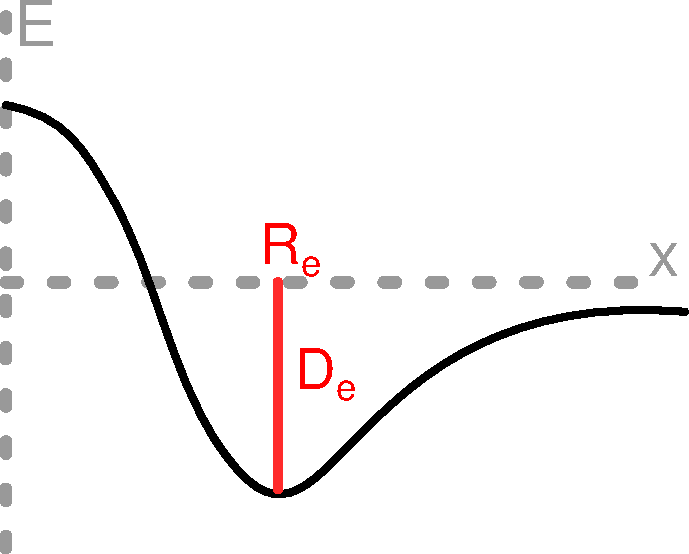
\includegraphics[scale=0.45]{schema1}

\subsection{Différentes types de laison}
C'est l'électronégativité qui contr\^ole le mode de partage des électroniques

	\begin{tabular}{_l^l^l}
		\tableHeaderStyle%
		Éléments & $\Delta \chi$ & Liaison\\
		Métal/Non métal & $>2.0$ & Ionique\\
		2 non métaux & $<0.6$ &Covalente non polarisée\\
		2 non métaux & $2.0>\Delta \chi >0.6$ & Covalente peu polarisée\\
		2 métaux & Faible & Métallique\\
		2 non métaux avec H & $\chi_A$ élevé& Hydrogène
	\end{tabular}

% \begin{itemize}
%  \item 2 non métaux d'électronégativité équivalente : Liaisons covalentes : Delta entre 0 et 0.4
%
% \item 2 non métaux d'électronégavité $\neq$ : Liaison covalente polarisées : Delta entre 0,4 et 2.0
%
% \item Un métal et un non métal d'électronégativité très différente : Liaison ionique : Transfert presque complet du lithium vers le Fluor. : Delta entre 2.0 et 4.0
%
% \item Un métal et un non métal d'électronégativité assez proche : Laison de coordination
%
% \item 2 métaux : Liaison métallique : Delta toujours faible
% \end{itemize}
\section{Construire une formule de Lewis}
\subsection{Travail préliminaire}
On compte le nombre total d'électrons de Valence de la molécule. On utilise la formule, avec $N_v(a)$ est le nombre d'électrons de Valence de l'atome $a$ et $z$ le nombre d'électrons en plus ou en moins dans le cas d'un ion.\marginCheck{Pour CO$^{2-}_3$, $z$ vaut $+2$ et pour NH$^+_4$, il vaut $-1$} :
\[N_e = \sum_a N_v(a)+z\]

Pour trouver le nombre de doublets, on divise par 2 si $N_e$ est pair ou on soustrait 1 et on divise par 2 dans le cas contraire.
\subsection{Écriture}
\subsubsection{Assemblage}
On écrit les atomes avec leur doublets non liants, puis on tente de les assembler.
\subsubsection{Règle de l'octet}
L'assemblage doit respecter la règle de l'octet pour les atomes $C,H,O,N$ au moins.\marginCritical{Les atomes à partir de la 3e période peuvent devenir hypervalents : ils sont alors entourés de plus d'un octet d'électrons.}


\subsection{Charge formelle}
On définit le nombre apparent d’électrons $N_a$ autour de chaque atomes de l’édifice en se fondant sur les règles suivantes :\marginCritical{
Cette façon de compter est différente de la manière de compter les électrons pour vérifier la règle de l'octet.}
\begin{itemize}
 \item Les électrons de tout doublet non liant appartiennent en propre
à l’atome.
\item Les électrons d’un doublet liant sont équitablement partagés
entre les deux atomes concernés par la liaison.
\end{itemize}
Si $N_a > N_v$, on rajoute une charge formelle $\ominus$ sur l'atome

Si $N_a < N_v$, on rajoute une charge formelle $\oplus$ sur l'atome

On fait porter la charge partielle - sur l'atome le plus électronégatif.
Souffre  = 6 liaisons
P = 5
\warningInfo{Somme des charges formelles}{La somme des charges formelles soit \^etre égale à celle de la molécule}
\subsection{Mésomérie}
Pour certaines molécules, il y a plusieurs schémas de Lewis possible. Ces représentations de Lewis s'appellent des formes mésomères. La molécule évolue contin\^ument entre ces dernières.

\subsubsection{Conséquences sur les longueurs et les énergies de liaison}
Si 2 liaisons changent continuellement entre liaison simple et liaison double, elles ont des propriétés intermédiaires entre celles des liaisons simples et celles des liaisons doubles, concernant leur longueur mais aussi leur énergie.
\subsubsection{Forme la plus probable}
\begin{theorem}[Règles des formes probables]
\begin{enumerate}
 \item Les représentations de Lewis qui décrivent les configurations les
plus stables d’un édifice chimique sont celles qui possèdent le moins de charges formelles possibles.
\item Les plus stables seront celles qui attribuent les charges négatives aux atomes les plus électronégatifs et les charges positives au atomes les moins électronégatifs.
\end{enumerate}
\end{theorem}
\subsection{Exemptions à la règle de l'octet}
\subsubsection{Radicaux}
Les molécules avec un nombre impair d'électrons de Valence, i.e. avec un électron célibataire.
\subsubsection{Molécules avec des lacunes électroniques}
C'est le cas du $Be, B, Li$. Ils possèdent des OA vides que l'on symbolise par des rectangles.
\subsubsection{Atomes hypervalents}
Seuls les atomes à partir de la 3e période peuvent l'\^etre. C'est le cas du $P$, qui est pentavalent et du $S$ qui est hexavalent.



\section{Géométrie des molécules}
Les strcutures de Lewis ne donnent aucune information sur la géométrie de la molécule.
\subsection{Méthode VSEPR}
On minimise la répulsion entre paires électroniques.

La géométrie la plus stable est celle où la répulsion entre doublets est minimisé au maximum.
\begin{enumerate}
 \item Elle s'applique autour d'un atome central ou de plusieurs atomes centraux.
\item On prend le nomre de liaisons covalentes (toutes liaisons multiples comptent pour 1) (n) et le nombre de NDL (m)
\item On obtient la catégorie molécule : $AX_nE_m$
\item On obtient les figures de répulsion
\item Géométrie = figure de répulsion en ignorant les doublets non liants.\marginInfo{Pour voir les liens entre figure de répulsion géométrie et catégorie, voir les cartes de révision associées à cette ressource.}
\end{enumerate}
\subsection{Angles et doubles liaisons}
Une liaison double repousse un peu plus que des liaisons simples, tout comme une triple repousse plus qu'une double

Les doublets non liants repoussent plus que ceux liants

Le modèle marche donc bien à quelques degrés près


\section{Liaisons}
\subsection{Liaisons de coordination}
Elles se produisent entre des atomes présentant une lacune électronique (acide de Lewis) et un atome avec un Doublet non liant (base de Lewis).
\subsection{Liaisons polarisées et moment dipolaire}
Des liaisons peuvent \^etre à la fois ioniques et covalentes : liaisons iono-covalentes

Les 2 atomes forment un dipole permanent et un moment dipolaire (de la charge - vers +, dans la direction des 2 atomes et de norme $q\times R$ avec $R$ la distance entre les atomes et $q$.\marginQuestion{On ne mesure pas $q$ mais le moment dipolaire de façon expérimentale.}. Elle s'exprime en Debye.

\subsection{Caractère Ionique Partiel}
$100\times \frac{\mu_{exp}}{\mu_{TC}}$ : C'est le rapport entre le moment dipolaire réel et le moment dipolaire théorique si l'on transfère 100\% des électrons.

\marginInfo{On calcule au numérateur la norme du vecteur avec la charge (1eV car transfert d'électron complet) multiplié par la distance (donnée) et on divise pour obtenir un résultat en Debye et non en C$\cdot$m.}

\begin{theorem}[Calculer $\mu_{TC}$]
\[\mu_{TC} = \frac{1.6\times 10^{-19} \times R}{3.336\cdot 10^{-30}}\] avec $1.6\times 10^{-19}$ 1 eV et $3.336\cdot 10^{-30}$ pour obtenir le résultat en Debye.
\end{theorem}
Exemple : $HF$ : $\mu_{TC} \frac{1.6\times 10^{-19} \times (92\times 10^{-12})}{3.336\cdot 10^{-30}} = 4.4D$

CIP = $100\times \frac{1.8}{1.4}$
\subsubsection{Évolution}
Une différence d'électronégativité plus importante entre les 2 éléments liés fait que le CIP sera plus élevé. Le moment dipolaire diminue car les distances diminuent.\marginInfo{Par exemple, on peut s'attendre à ce que le moment dipolaire entre $N$ et $O$ soit plus faible qu'entre $O$ et $H$ car la différence d'électronégativité est plus faible.}
\section{Liaisons}
\subsection{Liaisons hydrogènes}
\begin{theorem}[Définition]
Entre 2 molécules : un atome électronégatif portant des DNL et un hydrogène. Ce sont des liaisons faibles en énergie. Plus l'électronégativité de l'atome est haute, plus la liaison sera forte
\end{theorem}
Il faut que la molécule possède un moment dipolaire. Cela à des conséquences sur la vitesse de propagation des ions dans l'eau.\marginInfo{Diffusion hydrodynamique dans l'eau pour la majorité des molécules. Mais liaison structurante pour l'Hydrogène qui se propage à travers les molécules m\^eme}
\subsection{Liaisons de Van des Waals}
Entre atomes ou molécules et sont d'origine électrostatique. Il y en a 3 types :
\begin{itemize}
 \item Entre dipoles permanent, molécules polaires (faible par rapport à une liaison hydrogène)
 \item Entre un dipole permanant et une molécule polarisable (dipole induit)
 \item Entre molécules polarisable (dipoles instantanés), sans moment dipolaire. Mais les nuages proches entre eux vont se polariser mutuellement (très très faible)
\end{itemize}
\end{document}

